% В этом документе преамбула

\documentclass[a4paper,12pt]{article}

\usepackage{lscape} % горизонтальный режим
\usepackage{pdflscape}

\usepackage{lipsum} % тестовые тексты

%%% Работа с русским языком
\usepackage{cmap}					% поиск в PDF
\usepackage{mathtext} 				% русские буквы в формулах
\usepackage[T2A]{fontenc}			% кодировка
\usepackage[utf8]{inputenc}			% кодировка исходного текста
\usepackage[english,russian]{babel}	% локализация и переносы
\usepackage{indentfirst}			% чтобы первый абзац в разделе отбивался красной строкой
\frenchspacing						% тонкая настройка пробелов
\usepackage{gensymb}				% символы по типу градусов
\usepackage{algorithm}				% для алгоритмов
\usepackage{algorithmic}			% для алгоритмов

%%% Приведение начертания букв и знаков к русской типографской традиции
\renewcommand{\epsilon}{\ensuremath{\varepsilon}}
\renewcommand{\phi}{\ensuremath{\varphi}}			% буквы "эпсилон"
\renewcommand{\kappa}{\ensuremath{\varkappa}}		% буквы "каппа"
\renewcommand{\le}{\ensuremath{\leqslant}}			% знак меньше или равно
\renewcommand{\leq}{\ensuremath{\leqslant}}			% знак меньше или равно
\renewcommand{\ge}{\ensuremath{\geqslant}}			% знак больше или равно
\renewcommand{\geq}{\ensuremath{\geqslant}}			% знак больше или равно
\renewcommand{\emptyset}{\varnothing}				% знак пустого множества

%%% Дополнительная работа с математикой
\usepackage{amsmath,amsfonts,amssymb,amsthm,mathtools,esint} % AMS
\usepackage{wasysym}
\usepackage{icomma} % "Умная" запятая: $0,2$ --- число, $0, 2$ --- перечисление

%% Номера формул
\mathtoolsset{showonlyrefs=true} % Показывать номера только у тех формул, на которые есть \eqref{} в тексте.

%% Свои команды

% операции, не определённые (или имеющие иные обохначения) в мат. пакетах
\DeclareMathOperator{\sgn}{\mathop{sgn}}				% ф-ия sgn
\renewcommand{\tg}{\mathop{\mathrm{tg}}\nolimits}		% обозначение тангенса

%% Перенос знаков в формулах (по Львовскому)
\newcommand*{\hm}[1]{#1\nobreak\discretionary{}
{\hbox{$\mathsurround=0pt #1$}}{}}

%%% Работа с картинками
\usepackage{graphicx}  				% Для вставки рисунков
\graphicspath{{images/}{images2/}}  % папки с картинками
\setlength\fboxsep{3pt} 			% Отступ рамки \fbox{} от рисунка
\setlength\fboxrule{1pt} 			% Толщина линий рамки \fbox{}
\usepackage{wrapfig} 				% Обтекание рисунков текстом

%%% Работа с таблицами
\usepackage{array,tabularx,tabulary,booktabs} 	% Дополнительная работа с таблицами
\usepackage{longtable}  						% Длинные таблицы
\usepackage{multirow}							% Слияние строк в таблице

%%% Теоремы

\newtheoremstyle{break}% name
	{}%         Space above, empty = `usual value'
	{}%         Space below
	{\itshape}% Body font
	{}%         Indent amount (empty = no indent, \parindent = para indent)
	{\bfseries}% Thm head font
	{.}%        Punctuation after thm head
	{\newline}% Space after thm head: \newline = linebreak
	{}%         Thm head spec
\theoremstyle{break}

% \theoremstyle{plain} % Стиль по умолчанию
\newtheorem{theorem}{Теорема}[section]
\newtheorem{lemma}{Лемма}[section]
\newtheorem{definition}[theorem]{Определение}
\newtheorem{property}{Свойство}
 
\newtheorem{corollary}{Следствие}[theorem]

\newtheoremstyle{example}	% style name
	{2ex}					% above space
	{2ex}					% below space
	{}						% body font
	{}						% indent amount
	{\bf}				% head font
	{.}						% post head punctuation
	{\newline}				% post head punctuation
	{\thmname{#1}\thmnumber{ #2}\thmnote{ (#3)}}						% head spec

\theoremstyle{example}
\newtheorem{exmp}{Пример}[section]
 
\theoremstyle{remark} % "Примечание"
\newtheorem*{nonum}{Решение}
\newtheorem*{evidence}{Доказательство}
\newtheorem*{remark}{Примечание}

%%% Программирование
\usepackage{etoolbox} % логические операторы

%%% Страница
\usepackage{extsizes} % Возможность сделать 14-й шрифт
\usepackage{geometry} % Простой способ задавать поля
	\geometry{top=15mm}
	\geometry{bottom=35mm}
	\geometry{left=10mm}
	\geometry{right=10mm}

%\usepackage{fancyhdr} % Колонтитулы
% 	\pagestyle{fancy}
 	%\renewcommand{\headrulewidth}{0pt}  % Толщина линейки, отчеркивающей верхний колонтитул
% 	\lfoot{Нижний левый}
% 	\rfoot{Нижний правый}
% 	\rhead{Верхний правый}
% 	\chead{Верхний в центре}
% 	\lhead{Верхний левый}
%	\cfoot{Нижний в центре} % По умолчанию здесь номер страницы

\usepackage{setspace} % Интерлиньяж (межстрочные интервалы)
%\onehalfspacing % Интерлиньяж 1.5
%\doublespacing % Интерлиньяж 2
%\singlespacing % Интерлиньяж 1

\usepackage{lastpage} % Узнать, сколько всего страниц в документе.

\usepackage{soulutf8} % Модификаторы начертания

\usepackage{hyperref}
\usepackage[usenames,dvipsnames,svgnames,table,rgb]{xcolor}
\hypersetup{				% Гиперссылки
    unicode=true,           % русские буквы в раздела PDF
    pdftitle={Заголовок},   % Заголовок
    pdfauthor={Автор},      % Автор
    pdfsubject={Тема},      % Тема
    pdfcreator={Создатель}, % Создатель
    pdfproducer={Производитель}, % Производитель
    pdfkeywords={keyword1} {key2} {key3}, % Ключевые слова
    colorlinks=true,       	% false: ссылки в рамках; true: цветные ссылки
    linkcolor=MidnightBlue, % внутренние ссылки
    citecolor=black,        % на библиографию
    filecolor=magenta,      % на файлы
    urlcolor=blue           % на URL
}

\usepackage{csquotes} % Еще инструменты для ссылок

%\usepackage[style=authoryear,maxcitenames=2,backend=biber,sorting=nty]{biblatex}

\usepackage{multicol} % Несколько колонок

%%% Работа с графикой
\usepackage{tikz}
\usetikzlibrary{calc}
\usepackage{tkz-euclide}
\usetikzlibrary{arrows}
\usepackage{pgfplots}
\usepackage{pgfplotstable}

%%% Настройка подписей к плавающим объектам
% \usepackage{floatrow}	% размещение
\usepackage{caption}	% начертание
\captionsetup[figure]{labelfont=bf,textfont=it,font=footnotesize}	% нумерация и надпись курсивом
% для подфигур: заголовок подписи полужирный, текст заголовка обычный
% выравнивание является неровным (т.е. выровненным по левому краю)
% singlelinecheck = off означает, что настройка выравнивания используется, даже если заголовок имеет длину только одну строку.
% если singlelinecheck = on, то заголовок всегда центрируется, когда заголовок состоит только из одной строки.
\captionsetup[subfigure]{labelfont=bf,textfont=normalfont,singlelinecheck=off,justification=raggedright}

%%% Stuff для листинга
\usepackage{listings}
\usepackage{xcolor}

\colorlet{mygray}{black!30}
\colorlet{mygreen}{green!60!blue}
\colorlet{mymauve}{red!60!blue}

\lstset{
	backgroundcolor=\color{gray!10},  
	basicstyle=\ttfamily,
	columns=fullflexible,
	breakatwhitespace=false,      
	breaklines=true,                
	captionpos=b,                    
	commentstyle=\color{mygreen}, 
	extendedchars=true,              
	frame=single,                   
	keepspaces=true,             
	keywordstyle=\color{blue},      
	language=c++,                 
	numbers=none,                
	numbersep=5pt,                   
	numberstyle=\tiny\color{blue}, 
	rulecolor=\color{mygray},        
	showspaces=false,               
	showtabs=false,                 
	stepnumber=5,                  
	stringstyle=\color{mymauve},    
	tabsize=3,                      
	title=\lstname                
}

% для извращённых начертаний
\usepackage{mathrsfs}

\usepackage{makecell}
\setcellgapes{3pt}

% Зачёркивание символов
\usepackage{cancel}

% перечисления с буквами
\usepackage{enumitem}

\DeclareMathOperator{\eq}{\Leftrightarrow}
\DeclareMathOperator\supp{supp}

\title{Теория вероятностей и мат. статистика}
\date{11.04.2020}
\author{Почаев Никита Алексеевич, гр. 8381 \\ \href{mailto:pochaev.nik@gmail.com}{pochaev.nik@gmail.com} \\ Преподаватель: Малов Сергей Васильевич}

\begin{document}
	
\renewcommand{\figurename}{Рисунок}

\maketitle

\section*{Распределение функций он случайно величины}

\subsection*{Задача №7}

\begin{center}
	\fbox{%
		\parbox[t][4cm]{13cm}{%
			Пусть $\xi$ - случайная величина. Задача: найти распределение $\eta = f(\xi)$.
			
			Используем определение:
			\[ F_{\xi} = p(\xi < x) \text{ для любой с. величины } \xi \]
			
			Тогда:
			\[ F_{\eta} = p(\eta < x) = p(\xi \in f^{-1} (-\infty, x)), \text{ где} \] 
			\[f^{-1}(-\infty, x) = \{ y: f(y) \in (-\infty, x) \} \]
	}}\qquad
\end{center}

Определить распределение величины $\eta = G(\xi)$:
\begin{enumerate}
	\item[а)] если
	\[
	F_{\xi}(x) =
	\begin{cases}
		0, &x \le -2 \\
		\frac{1}{8}, &x \in (-2, -1] \\
		\frac{1}{3}, &x \in (-1, 0] \\
		\frac{1}{2}, &x \in (0, 2] \\
		1, &x > 2
	\end{cases}
	\]
	\[ G(t) = t^4 - t^2 + 2, t \in \mathbb{R} \]
	\item[б)] если
	\[
	F_{\xi}(x) =
	\begin{cases}
		0, &x \le 1 \\
		1 - \frac{1}{n}, &x \in (n-1, n], n = 1,2,\dots
	\end{cases}
	\]
	\[ G(t) = \sin \pi t, t \in \mathbb{R} \]
\end{enumerate}

\noindent\textit{Решение:}

\begin{enumerate}
	\item[а)] Соотношение между возможными значениями случайной величины и их вероятностями называется законом распределения дискретной случайной величины (ДСВ). Запишем его в виде таблицы:
	\begin{table}[H]
		\centering\makegapedcells
		\begin{tabular}{|c|c|c|c|c|}
			\hline
			$k$        & -2            & -1                                         & 0                                     & 2             \\ \hline
			$P(\xi=k)$ & $\frac{1}{8}$ & $\frac{1}{3} - \frac{1}{8} = \frac{5}{24}$ & $\frac{1}{2}-\frac{1}{3}=\frac{1}{6}$ & $\frac{1}{2}$ \\ \hline
		\end{tabular}
	\end{table}
	Проверка: $ p(\xi \in [0,1]) = \sum\limits_{i=1}^{n}p_i = 1$
	
	Посмотрев на функцию $G(\xi)$ заключаем, что она является чётной: $G(-t) = (-t)^4 - (-t)^2 + 2 = G(t)$.
	
	Вычислим значения функции величины $\eta = G(\xi)$:
	\begin{itemize}
		\item $\xi = 2, G(2) = G(-2) = 16 - 4 + 2 = 14 \Rightarrow p(\eta = 14) = \frac{1}{8} + \frac{1}{2} = \frac{5}{8}$
		\item $\xi = -1, G(-1) = 2$ аналогично $\xi = 0, G(0) = 2 \Rightarrow p(\eta = 2) = \frac{5}{24} + \frac{1}{6} = \frac{3}{8}$
	\end{itemize}
	Таким образом, функция распределение величины $\eta$ имеет следующий вид:
	\[
	F_{\eta}(x) =
	\begin{cases}
		0, &x \le 2 \\
		\frac{3}{8}, &x \in (2, 14] \\
		\frac{5}{8} + \frac{3}{8} = 1, &x > 14
	\end{cases}
	\]
	График ($F_{\xi}$ - красный, $F_{\eta}$ - синий)
	\begin{figure}[H]
		\center{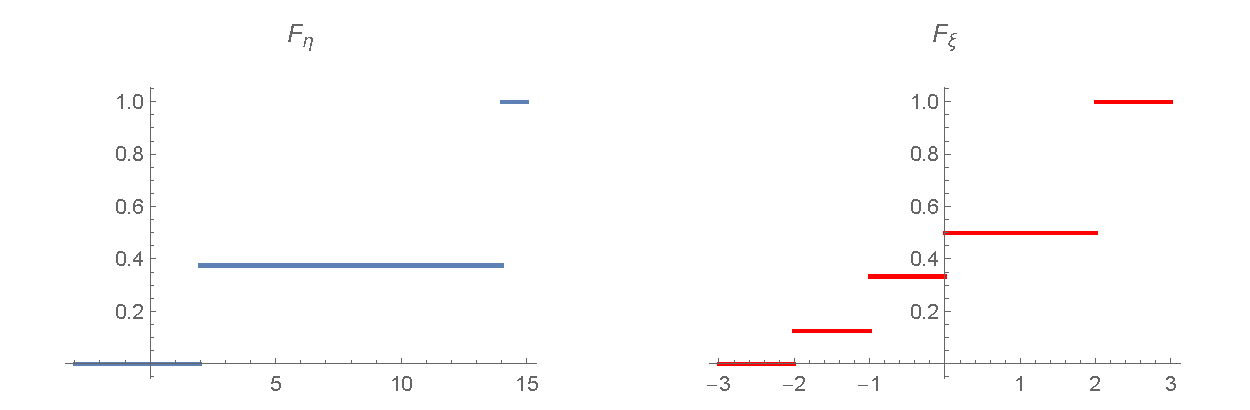
\includegraphics[scale=0.9]{./media/11_04_20_1.pdf}}
	\end{figure}
	\item[б)] Аналогично предыдущему пункту, представим распределение в виде таблицы:
	\begin{table}[H]
		\centering\makegapedcells
		\begin{tabular}{|c|c|c|c|c|c|c|c|}
			\hline
			$k$        & $n$                                              & 1             & 2             & 3              & 4              & 5              & $\dots$ \\ \hline
			$P(\xi=k)$ & $\cancel{1}-\frac{1}{n+1}-\cancel{1}+\frac{1}{n}=\frac{1}{n(n+1)}$ & $\frac{1}{2}$ & $\frac{1}{6}$ & $\frac{1}{12}$ & $\frac{1}{20}$ & $\frac{1}{30}$ & $\dots$ \\ \hline
		\end{tabular}
	\end{table}
	Для любой с. величины $\xi: \eta = G(\xi) = \sin \pi \xi = 0$ (т.к. на какой коэффициент $\in \mathbb{R}$ мы не домножим, всё равно значение синуса будет лежать на оси абсцисс). Следовательно,
	\[ p(\eta = 0) = \sum_{i=1}^{\infty} p(\xi = i) = 1 \]
	Таким образом, функция распределение величины $\eta$ имеет следующий вид:
	\[
	F_{\eta} =
	\begin{cases}
		0, &x \le 0 \\
		1, &x > 0
	\end{cases}
	\]

\end{enumerate}

\subsection*{Задача №8}

\begin{center}
	\fbox{%
		\parbox[t][4cm]{13cm}{%
			Носитель функции $u: X \to \mathbb{R}$ — это замыкание подмножества $X$, на котором вещественно-значная функция $u$ не обращается в ноль:
			\[ \supp u = \overline{\{x|u(x) \ne 0\}} \]
			
			\[ p(\xi \in [0,1]) = 1,  \]
			\[ \supp (\xi) = [0,1] \Rightarrow \supp (\eta) = [-\infty, \infty] \]
	}}\qquad
\end{center}

Вычислить распределение величины $\eta = G(\xi)$, если величина $\xi$ имеет плотность распределения:
\begin{enumerate}
	\item[а)]
	\[
	p_{\xi} =
	\begin{cases}
		|x|, x \in [-1,1] \\
		0 - \text{ в остальных случаях}
	\end{cases}
	\]
	\[ G(t) = t^2 - 1 \]
	
	$p(\xi \in [-1,1]) = 1$, т.е. $\supp (\xi) = [-1,1] \Rightarrow \supp (\eta = G(\xi)) = [-1,0]$, 
	
	т.к. $G(-1) = 1 - 1 = 0$ и $G(0) = 0 - 1 = -1$.
	\[ F_{\eta} = P(\eta < x) = p(\xi^2 - 1 < x) \underset{\text{реш. нер-во}}{=} p(\xi^2 < x + 1) = p(|\xi| < \sqrt{x+1}) (\text{по опр., см. табл. 1-ый пункт}) \]
	
	Заметим, что по опр. функции модуля, ф-ия $p_{\xi}(x)$ явл-ся чётной, как следствие,
	\[ F_{\eta}(x) = \int_{-\sqrt{x+1}}^{\sqrt{x+1}} |t|dt =2 \int_{0}^{\sqrt{x+1}}t dx = x+1 \text{ для } x \in (-1,0] \color{gray}(\Re(x) \le -1 \land \Im(x) = 0) \]
	Таким образом, величина $\xi$ имеет следующее распределение:
	\[
	F_{\eta}(x) =
	\begin{cases}
		0, &x \le -1 \\
		x + 1, &x \in (-1,0] \\
		1, &x > 0
	\end{cases}
	\]
	Дифференцируя функцию распределения, получаем плотность распределения:
	\[
	p_{\eta} (x) =
	\begin{cases}
		0, &x \notin [-1,0] \\
		1, &x \in [-1,0]
	\end{cases}
	\]
	
	\item[б)]
	\[
	p_{\xi}(x) = \frac{1}{\sqrt{2 \pi}}\exp\left(-\frac{x^2}{2}\right), x \in \mathbb{R}, G(t) = at + b, t \in \mathbb{R}, a,b - const
	\]
	
	В данном случае величина $\xi$ и отображение $G$ абсолютно непрерывны и $G$ монотонна (знак её производной определяется знаком константы $a: G'(t)=a$), следовательно, можно применить следующую формулу, связывающую плотности распределения $\xi$ и $\eta$:
	\[ p_{\eta} (x) = p_{\xi} (G^{-1}(x)) | (G^{-1})'(x)| \text{ для почти всех } x \in \mathbb{R} \]
	\[ G^{-1}(x) = \frac{x-b}{a}; (G^{-1})'(x) = \frac{1}{a} \]
	\[ p_{\eta}(x) = \frac{1}{|a|} p_{\xi} \left(\frac{x-b}{a}\right) = \frac{1}{|a|\sqrt{2 \pi}} \exp \left(-\frac{(x-b)^2}{2a^2}\right) \]
	
	\item[в)]
	\[
	p_{\xi}(x) =
	\begin{cases}
		\frac{1}{2} \sin x, x \in [0, \pi] \\
		0 - \text{ в остальных случаях}
	\end{cases}
	\]
	\[ G(t) = \cos t, t \in \mathbb{R} \]
	
	Посмотрев на ф-ию распределения, заключаем, что носитель распределения $\xi$ совпадает с интервалом $[0,\pi]$. Образ данного интервала при отображении "косинус"\, совпадает с интервалом $[-1,1]$. Следовательно, $F_{\eta}(x) = 0$ при $x \le -1$, $F_{\eta}(x) = 1$ при  $x > 1$.
	\[ p(\xi \in [0,\pi]) = 1 \Rightarrow \supp (\xi) = [0,\pi] \Rightarrow \supp (\eta = G(\xi)) = [-1,1] \]
	\[
	F_{\xi}(x) =
	\begin{cases}
		0, &x \le 0 \\
		\int_{0}^{x} \frac{1}{2} \sin t dt = \sin^2 \left(\frac{x}{2}\right), &x \in (0,\pi] \\
		1, &x > \pi
		\end{cases}
	\]
	\[ F_{\eta}(x) = P(\eta < x) = p(\cos \xi < x) = p(\xi > \arccos x) = \int_{\arccos x}^{\pi} \frac{1}{2} \sin t dt =\] 
	\[ = - \frac{\cos x}{2} \bigg|_{\arccos x}^{\pi} = \frac{x+1}{2} \]
	Таким образом, функция распределения:
	\[
	F_{\eta} =
	\begin{cases}
		0, &x \le -1 \\
		\frac{x+1}{2}, x \in (-1,1] \\
		1, &x > 1
	\end{cases}
	\]
	Дифференцируя функцию распределения, получаем плотность распределения:
	\[
	p_{\eta}(x) =
	\begin{cases}
		\frac{1}{2}, x \in [-1,1] \\
		0 - \text{ в остальныных случаях}
	\end{cases}
	\]
	
	\item[г)]
	\[ p_{\xi} = \frac{1}{2} \exp (-|x|), x \in \mathbb{R}, G(t) = t^2, t \in \mathbb{R} \]
	
	Носитель распределения будет совпадать с интервалом $\supp (\eta) = [0, +\infty)$. Следовательно, $F_{\eta}(x) = 0$ при $x \le 0$. При $x>0$:
	\[ F_{\eta} (x) = \int_{-\sqrt{x}}^{\sqrt{x}} p_{\xi} (t)dt = s \int_{0}^{\sqrt{x}} \frac{1}{2} \exp (-t)dt = 1 - \exp (- \sqrt{x}) \]
	Таким образом, величина $\xi$ имеет следующее распределение:
	\[
	F_{\eta}(x) =
	\begin{cases}
		0, &x \le 0 \\
		1 - \exp (-\sqrt{x}), &x > 0
	\end{cases}
	\]
	Дифференцируя функцию распределения, получаем плотность распределения:
	\[
	p_{\eta}(x) =
	\begin{cases}
		0, &x \le 0 \\
		\frac{\exp (- \sqrt{x})}{2\sqrt{x}}, &x > 0
	\end{cases}
	\]
\end{enumerate}

\end{document} 